\documentclass{article}

\usepackage{fancyhdr}
\usepackage{extramarks}
\usepackage{amsmath}
\usepackage{amsthm}
\usepackage{amsfonts}
\usepackage{tikz}
\usepackage[plain]{algorithm}
\usepackage{algpseudocode}
\usepackage{listings}
\usepackage{minted}
\usepackage[utf8]{inputenc}
\usepackage[english]{babel}
\usetikzlibrary{automata,positioning}
\usepackage{graphicx}
%
% Basic Document Settings
%


\topmargin=-0.45in
\evensidemargin=0in
\oddsidemargin=0in
\textwidth=6.5in
\textheight=9.0in
\headsep=0.25in

\linespread{1.1}

\pagestyle{fancy}
\lhead{\hmwkClass\ (\hmwkClassInstructor): \hmwkTitle}
\chead{\hspace{4.8in}\hmwkAuthorName}
\rhead{\firstxmark}
\lfoot{\lastxmark}
\cfoot{\thepage}

\renewcommand\headrulewidth{0.4pt}
\renewcommand\footrulewidth{0.4pt}

\setlength\parindent{0pt}

%
% Create Problem Sections
%

\newcommand{\enterProblemHeader}[1]{
    \nobreak\extramarks{}{Problem \arabic{#1} continued on next page\ldots}\nobreak{}
    \nobreak\extramarks{Problem \arabic{#1} (continued)}{Problem \arabic{#1} continued on next page\ldots}\nobreak{}
}

\newcommand{\exitProblemHeader}[1]{
    \nobreak\extramarks{Problem \arabic{#1} (continued)}{Problem \arabic{#1} continued on next page\ldots}\nobreak{}
    \stepcounter{#1}
    \nobreak\extramarks{Problem \arabic{#1}}{}\nobreak{}
}

\setcounter{secnumdepth}{0}
\newcounter{partCounter}


%
% Homework Problem Environment
%
% This environment takes an optional argument. When given, it will adjust the
% problem counter. This is useful for when the problems given for your
% assignment aren't sequential. See the last 3 problems of this template for an
% example.
%


%
% Homework Details
%   - Title
%   - Due date
%   - Class
%   - Section/Time
%   - Instructor
%   - Author
%

\newcommand{\hmwkTitle}{Homework 2}
\newcommand{\hmwkDueDate}{Tuesday, Feb 16, 2016}
\newcommand{\hmwkClass}{DS-GA 1003}
\newcommand{\hmwkClassInstructor}{Professor David Ronsenberg}
\newcommand{\hmwkAuthorName}{Yuhao Zhao}
\newcommand{\hmwknetid}{Yz3085}
\newcommand{\hmwksubtitle}{Lasso}

%
% Title Page
%

\title{
    \vspace{2in}
    \textmd{\textbf{\hmwkClass:\ \hmwkTitle \\ \hmwksubtitle }}\\
    \vspace{1in}
    \normalsize\vspace{0.1in}\small{Due\ on\ \hmwkDueDate}\\
    \vspace{0.1in}\large{\textit{\hmwkClassInstructor}}
    \vspace{3in}
}

\author{\textbf{\hmwkAuthorName} \\ \textbf{\hmwknetid }}
\date{}

\renewcommand{\part}[1]{\textbf{\large Part \Alph{partCounter}}\stepcounter{partCounter}\\}

%
% Various Helper Commands
%

% Useful for algorithms
\newcommand{\alg}[1]{\textsc{\bfseries \footnotesize #1}}

% For derivatives
\newcommand{\deriv}[1]{\frac{\mathrm{d}}{\mathrm{d}x} (#1)}

% For partial derivatives
\newcommand{\pderiv}[2]{\frac{\partial}{\partial #1} (#2)}

% Integral dx
\newcommand{\dx}{\mathrm{d}x}

% Alias for the Solution section header
\newcommand{\solution}{\textbf{\large Solution}}

% Probability commands: Expectation, Variance, Covariance, Bias
\newcommand{\E}{\mathrm{E}}
\newcommand{\Var}{\mathrm{Var}}
\newcommand{\Cov}{\mathrm{Cov}}
\newcommand{\Bias}{\mathrm{Bias}}


\newenvironment{problem}[2][$\bullet$]{\begin{trivlist}\large
		\item[\hskip \labelsep {\bfseries #1}\hskip \labelsep {\bfseries #2.}]}  {\end{trivlist}}

\newenvironment{sub}[2][$-$]{\begin{trivlist}
		\item[\hskip \labelsep {\bfseries #1}\hskip \labelsep {\bfseries #2.}]}  {\end{trivlist}}
\newenvironment{lemma}[2][Lemma]{\begin{trivlist}
		\item[\hskip \labelsep {\bfseries #1}\hskip \labelsep {\bfseries #2.}]}{\end{trivlist}}
\newenvironment{exercise}[2][Exercise]{\begin{trivlist}
		\item[\hskip \labelsep {\bfseries #1}\hskip \labelsep {\bfseries #2.}]}{\end{trivlist}}

\newenvironment{question}[2][Question]{\begin{trivlist}
		\item[\hskip \labelsep {\bfseries #1}\hskip \labelsep {\bfseries #2.}]}{\end{trivlist}}
\newenvironment{corollary}[2][Corollary]{\begin{trivlist}
		\item[\hskip \labelsep {\bfseries #1}\hskip \labelsep {\bfseries #2.}]}{\end{trivlist}}

\begin{document}

\maketitle

\pagebreak


%\lstinputlisting{hw1_skeleton_code.py}

\section{1.Preliminaries }
\begin{problem}{\large{1.1 Feature Normalization}}
\end{problem}

\begin{sub}{1.1.1}
\end{sub}
\begin{minted}{python}
import numpy as np
import matplotlib.pyplot as plt
import time
from hw1 import *
from scipy.optimize import minimize
from sklearn.cross_validation import train_test_split
from sklearn.linear_model import Ridge

X = np.random.rand(150,75)
\end{minted}

\begin{sub}{1.1.2}
\end{sub}
\begin{minted}{python}
theta_true = 20*numpy.random.randint(2,size = 10)-10
theta_true = np.array([np.hstack((theta_true,np.zeros(65)))]).T
\end{minted}

\begin{sub}{1.1.3}
\end{sub}
\begin{minted}{python}
noise = np.array([0.1*np.random.randn(150)]).T
y = np.dot(X,theta_true) + noise
\end{minted}

\begin{sub}{1.1.4}
\end{sub}
\begin{minted}{python}
X_train_, X_test, y_train_, y_test = train_test_split(X, y, test_size =50, random_state=10)
X_train,X_validation,y_train,y_validation = 
	train_test_split(X_train_, y_train_, test_size =20, random_state=11)
\end{minted}

\vspace{0.2in}

\begin{problem}{\large{1.2 Experiment with Ridge Regression}}
\end{problem}

\begin{sub}{1.2.1}
\end{sub}
\begin{minted}{python}
temp = Ridge_lambda_search(X_train,y_train[:,0],X_validation,y_validation[:,0],
			lambda_ = np.power(10, np.linspace(-7,6,100)))[0]
lambda_opt = np.power(10, np.linspace(-7,6,100))[np.where(temp  ==np.nanmin(temp))[0][0]]
beta_= regularized_grad_descent(X_train,y_train[:,0],lambda_reg = lambda_opt )[0][-1,:]
np.sum(theta_true[10:,:] != np.array([beta_]).T[10:])


\end{minted}


According to the Ridge regression algorithm in assignment 1 (see code in appendix), the best $\lambda $ is $ 10^{-7}$. There are 65 components(every components) with true 0 but was estimated to be non-zero. None component with non-zero was estimated as zero.  \\

After thresholding by $10^{-3}$, there are still 65 components with true 0 but was estimated to be non-zero.

\pagebreak
\section{2 Coordinate Descent for Lasso (a.k.a The shooting algorithm)}
\begin{problem}{2.1 Experiments with the Shooting Algorithm}
\end{problem}

\begin{sub}{2.1.1}
\end{sub}

\begin{minted}{python}
def LassoShooting(X, y, lambda_ = 0.1,epsilon = 0.0001,n_iter = 1000,
				beta_init = np.zeros((X.shape[1],1)) ):
	"""
	input: Training data X, traing data label, regulization, converging criterion, 
	warm starting value for homotopy method.
	
	output: optimized beta and training error
	"""
	num_instances, num_features = X.shape      
	beta = beta_init
	t = 0
	converged = False
	Loss = np.linalg.norm(np.dot(X,beta) - y)**2 *(1.0/(2*num_instances))
	while (not converged and t <=n_iter ):
		beta_start = beta
		for j in range(num_features):
			aj = 0
			cj = 0
			for i in range(num_instances):
				aj += 2*X[i,j]**2
				cj += 2*X[i,j] *(y[i][0] - np.inner(beta_start[:,0],X[i,:])
								+beta_start[j][0]*X[i,j])
				
			beta[j] = np.sign(aj)* (lambda x: np.sign(x[0])* ((abs(x[0]) - x[1]) 
					if (abs(x[0]) - x[1])>0 else 0))([cj/aj,lambda_/aj])
		t+=1
		converged = abs(Loss - np.linalg.norm(np.dot(X,beta) - y)**2
					*(1.0/(2*num_instances))) < epsilon
		Loss = np.linalg.norm(np.dot(X,beta) - y)**2*(1.0/(2*num_instances))
	return (beta,Loss)

try_list =  np.power(10,np.linspace(0,2,30)) 
loss_hist = np.zeros(try_list.shape[0])

time1 = time.time()
for i,reg in enumerate(try_list):
	beta = LassoShooting(X_train,y_train,lambda_ = reg)[0]
	loss_hist[i] = np.linalg.norm(np.dot(X_validation,beta) - y_validation)**2
				*(1.0/(2*num_instances))
time_hist_1 = time.time()-time1 
\end{minted}
\begin{center}
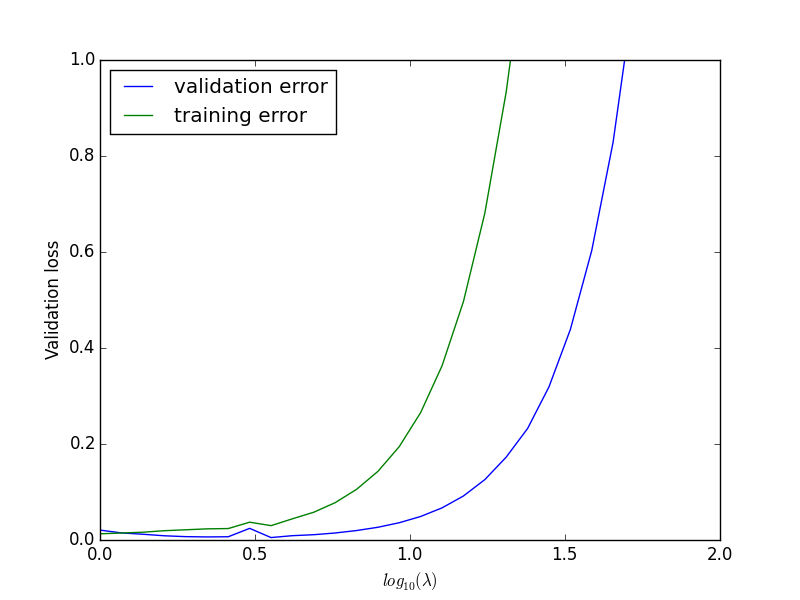
\includegraphics[height = 3.5in]{2_1.png}
\end{center}

The optimal $\lambda$ is 3.56224 and the corresponding test error is 0.11532799428214691
\\

\begin{sub}{2.1.2}
\end{sub}

\begin{minted}{python}
>>> np.sum(theta_true[10:,:] != beta_opt[10:,:])
>>> 2
>>>beta_opt[:10,:]
>>>array([[ -9.1941852 ],
array([[-9.92480386],
	[-9.7845817 ],
	[ 9.69160619],
	[-9.74515336],
	[-9.73290275],
	[ 9.6222794 ],
	[-9.81244892],
	[-9.81588341],
	[ 9.63381792],
	[ 9.78238686]])

\end{minted}

There are 2 components with true value zero that was estimated non-zero. None component with non-zero was estimated as zero.\\

\begin{sub}{2.1.3}
\end{sub}
\begin{minted}{python}
loss_hist_3 = np.zeros(try_list.shape[0])
pre = np.zeros((75,1))
time2 = time.time()
for i,reg in enumerate(try_list):
	beta = LassoShooting(X_train,y_train,lambda_ = reg,beta_init =pre )[0]
	pre,loss_hist[i] = beta, np.linalg.norm(np.dot(X_validation,beta) -
				 y_validation)**2*(1.0/(2*num_instances))
time2  = time.time() -time2
\end{minted}

The basic shooting algorithm takes 14.76 seconds and the homotopy method takes 17.2901 seconds.

\begin{sub}{2.1.4}
\end{sub}

\begin{minted}{python}
def LassoShooting_mat(X, y, lambda_ = 0.1,epsilon = 0.0001,n_iter = 1000,
			beta_init = np.zeros((X.shape[1],1)) ):
	"""
	input: Training data, training labels, regulization, converging criterion, 
	warm starting value for homotopy method.
		
	output: optimized beta and training error
	"""
	num_instances, num_features = X.shape      
	beta = beta_init
	t = 0
	converged = False
	XX2 = np.dot(X.T,X)*2;
	Xy2 = np.dot(X.T,y)*2
	Loss = np.linalg.norm(np.dot(X,beta) - y)**2*(1.0/(2*num_instances))
	while (not converged and t <=n_iter ):
		beta_start = beta
		for j in range(num_features):
			aj = XX2[j,j]
			cj = (Xy2[j] - np.dot(XX2[j,:],beta_start) + XX2[j,j]*beta_start[j])[0]
			beta[j] = np.sign(aj)* (lambda x: np.sign(x[0])* ((abs(x[0]) - x[1]) 
					if (abs(x[0]) - x[1])>0 else 0))([cj/aj,lambda_/aj])
		t+=1
		converged = abs(Loss - np.linalg.norm(np.dot(X,beta) - y)**2
					*(1.0/(2*num_instances))) < epsilon
		Loss = np.linalg.norm(np.dot(X,beta) - y)**2*(1.0/(2*num_instances))
	return (beta,Loss)

pre = np.zeros((75,1))
time3 = time.time()
for i,reg in enumerate(try_list):
	beta = LassoShooting_mat(X_train,y_train,lambda_ = reg,beta_init =pre )[0]
	pre,loss_hist[i] = beta, np.linalg.norm(np.dot(X_validation,beta) -
			y_validation)**2*(1.0/(2*num_instances))
time_hist_3 = time.time()-time3
\end{minted}

Since $a_j = 2\sum_{i=1}^{n} x^2_{ij}  =2\times x_{: j}^T \cdot x_{: j}$, which is 2 times $j,j $ th element of $X^TX$ matrix\\

$c_j  = 2\sum_{i=1}^{n} x_{ij}(y_i - w^Tx_i + w_jx_{ij}) = 2( \sum_{i=1}^{n} x_{ij} y_i - \sum_{i=1}^{n} w^Tx_i x_{ij} + \sum_{i=1}^{n}  w_jx_{ij} x_{ij} )$\\
$\sum_{i=1}^{n}  x_{ij} y_i$ is the jth column of X dot product with y, which is the jth element of $2X^Ty$\\
$ \sum_{i=1}^{n}  w^Tx_i x_{ij} $ is the jth row of $X^TX$ dot product with w\\
$\sum_{i=1}^{n}  w_jx_{ij} x_{ij} $ is $j,j $ th element of $X^TX$ matrix times the jth element of w\\
Therefore, $c_j = 2([X^Ty]_{j} + [X^TX]_{j:} \cdot w + w_j \times [X^TX]_{j,j})$ 

The running time for this matrix based expression is 0.476298 seconds which is much better than the previous ones.

\begin{problem}{2.2 Derive the Coordinate Minimizer for Lasso}
\end{problem}

\begin{sub}{2.1.1}
\end{sub}
If $x_{i,j} = 0$ for $i = 1,...,n$  $f(w_j) = \sum_i (y_i^2) +\lambda |w_j| + \lambda \sum_{k \neq j} |w_k| $\\
By taking derivative w.r.t $w_j$, the coordinate minimizer is $w_j = 0$


\begin{sub}{2.2.2}
\end{sub}
For $w_j \neq 0, $\\$$ \frac{\partial f}{\partial w_j} = \sum_i 2(w_j x_{i,j} + \sum_{k \neq j} w_k x_{i,k} -y_i )x_{i,j} + \lambda sign(w_j)$$
 $$= \sum_i 2w_j x^2_{i,j} - 2\sum x_{i,j} (y_i - \sum_{j\neq k} w_k x_{i,k}) + \lambda sign(w_j) = a_j w_j - c_j +\lambda sign(w_j)$$
 
 \begin{sub}{2.1.3}
 \end{sub}
For $w_j > 0, sign(w_j) = 1$, to solve $ \frac{\partial f}{\partial w_j} = 0$, we have: \\
$$ a_j w_j - c_j +\lambda = 0$$Then
$$w_j = \frac{1}{a_j}(-\lambda +c_j) = -\frac{1}{a_j}(\lambda - c_j)$$\\
$w_j < 0, sign(w_j) = -1$, similarly, $$ w_j = \frac{1}{a_j}(\lambda +c_j) $$ 

\begin{sub}{2.1.4}
\end{sub}
By definition, for $w_j = 0$ to be a minimizer, we have to show its  two-sided derivatives are non-negative at f(0).\\
$\lim\limits_{\epsilon \downarrow 0}\frac{f(\epsilon) -f(0)}{\epsilon} =\lim\limits_{\epsilon \downarrow 0} \frac{\sum_i (\epsilon x_{i,j} + \sum_{k \neq j} w_k x_{i,k} -y_i )^2 + \lambda |\epsilon| + \lambda \sum_{k\neq j} |w_k| - \sum_i ( \sum_{k \neq j} w_k x_{i,k} -y_i )^2 - \lambda \sum_{k\neq j} |w_k| }{\epsilon} \\ = \lim\limits_{\epsilon \downarrow 0}\frac{\sum_i (\epsilon^2 x^2_{i,j} +2\epsilon x_{i,j}\sum_{j\neq k } w_kx_{i,k} - y_i )+ \lambda \epsilon}{\epsilon}  = \lim\limits_{\epsilon \downarrow 0} \frac{\sum_i \epsilon^2 x^2_{i,j}}{\epsilon}  -c_j + \lambda = \lambda -c_j \geq 0 $\\
Then, we have $c_j \leq \lambda$  \\
Similarly, on the other side, $\lim\limits_{\epsilon \downarrow 0}\frac{f( - \epsilon) -f(0)}{\epsilon} =\lim\limits_{\epsilon \downarrow 0}\frac{\sum_i (\epsilon^2 x^2_{i,j} -2\epsilon x_{i,j}\sum_{j\neq k } w_kx_{i,k} - y_i )+ \lambda \epsilon}{\epsilon}= c_j + \lambda \geq 0 $\\
Then we have $c_j \geq - \lambda$\\
Therefore, $c_j  \in [-\lambda, \lambda]$ implies $w_j = 0$ is a minimizer. 

\begin{sub}{2.1.5}
\end{sub}
From 2.1.3 we know that for $w_j > 0$, we have the solution $w_j = \frac{1}{a_j} (c_j - \lambda)$, since $a_j  \geq 0,$ we have $c_j > \lambda $\\For $w_j < 0$, we have the solution $w_j = \frac{1}{a_j} (c_j + \lambda)$, since $a_j  \geq 0,$ we have $c_j <  -\lambda $\\
From 2.1.4,  we know that for $c_j \in [-\lambda, \lambda],$ the solution is $w_j = 0$\\
The minimizer is indeed 
\[
w_{j}=\begin{cases}
\frac{1}{a_{j}}\left(c_{j}-\lambda\right) & c_{j}>\lambda\\
0 & c_{j}\in[-\lambda,\lambda]\\
\frac{1}{a_{j}}\left(c_{j}+\lambda\right) & c_{j}<-\lambda
\end{cases}
\]
On the other hand, $soft(\frac{c_j}{a_j},\frac{\lambda}{a_j}) = 0$ for $c_{j}\in[-\lambda,\lambda]  , = \frac{1}{a_{j}}\left(c_{j}-\lambda\right)$ for $c_{j}>\lambda$ and $ = \frac{1}{a_{j}}\left(c_{j}+\lambda\right) $ for $ c_{j}<-\lambda$\\ . This expression is equivalent to the expression given in 2.\\

\section{3 Lasso Properties}

\begin{problem}{3.1 Deriving $\lambda_{max}$}
\end{problem}
\begin{sub}{3.1.1}
\end{sub}
Since $L(w) = (Xw - y)^T(Xw-y) +\lambda |w|_1$\\
$$L'(0,v)  = \lim\limits_{h \downarrow0 } \frac{L(vh) - L(0)}{h} = \frac{(hXv - y)^T(hXv  -y) + \lambda h |v|_1 - (-y)^T(-y)}{h}$$$$ =\lim\limits_{h \downarrow0 } \frac{h^2v^TX^TXv - 2hv^TX^Ty + y^Ty - y^Ty + \lambda h|v|_1}{h} = -2v^TX^Ty + \lambda |v|_1$$

\begin{sub}{3.1.2}
\end{sub}
In order for $w^*$ to be a minimizer, L(w) we must have non-negative directional derivative in any direction v. \\
$L'(0,v) \geq 0$, then $ -2v^TX^Ty + \lambda |v|_1 \geq 0 $.\\
$\lambda \geq \frac{2v^TX^Ty}{|v|_1} $
\begin{sub}{3.1.3}
\end{sub}
Since the lower bounds on $\lambda$ should  hold for all v, $\lambda > g(v) =\frac{2v^TX^Ty}{|v|_1} $ for all v. Since v is a directional vector, we constrain $||v||_{L2} = 1$\\
$|v|^2_1 = (|v_1| + |v_2| + ... + |v_n|)^2 \geq  (|v_1 + v_2 +... + v_n|)^2  \geq v_1^2 + v_2^2 +... + v_n^2 = 1$ and the equal sign occurs when $v_i = 1, v_j = 0 \forall j \neq i$\\
The maximum value for $f(v)$ therefore occurs when $v_i = 1$ where i is the index that $X^Ty$ has the largest absolute value at the ith index.\\  Therefore, $max(g(v)) =   2||X^Ty||_\infty $. This is equivalent to say $\lambda \geq 2||X^Ty||_\infty $\\
$\lambda_{max} = 2||X^Ty||_\infty $

\begin{sub}{3.1.4}
	\end{sub}
For model with bias, $L(w) = (Xw + b-y)^T(Xw+b-y) + \lambda ||w||_1$\\
$L'(0,v) = \lim\limits_{h \downarrow0 } \frac{L(vh) - L(0)}{h} = \frac{(hXv +b - y)^T(hXv +b -y) + \lambda h |v|_1 - (b-y)^T(b-y)}{h}\\  =\lim\limits_{h \downarrow0 } \frac{h^2v^TX^TXv + 2hv^TX^T(b-y)  + \lambda h|v|_1}{h}  =2v^TX^T(b-y)  + \lambda |v|_1 \geq 0$\\
Therefore, $\lambda \geq \frac{2v^TX^T(b-y)}{|v|_1 }$

\begin{problem}{3.2 Feature Correlation}
\end{problem}
\begin{sub}{3.2.1}
\end{sub}
Since $X_{.i}, X_{.j}$ are exactly the same, we can regard $\hat{\theta_i},\hat{\theta_j}$ as one parameter C. we want to solve  \\
Min$ |\hat{\theta_i}| +|\hat{\theta_j}|,$ s.t $ \hat{\theta_i} +\hat{\theta_j} = C$\\
We notice that to minimize the function, $\hat{\theta_i}, \hat{\theta_j}$ should have the same sign.



Now we solve C, C should be the j-th coefficient that was solved by removing the i-th column in X:\\
From Question 2, we know that:\\
$a_j = 2 \sum_m x^2_{m,j}, c_j = 2 \sum_m x_{mj}(y_m - \sum_{k \neq j \neq i} w_kx_{m k}) $ \\
Therefore, depends on the value of $c_j$, \[
\hat{\theta_i} +\hat{\theta_j} =\begin{cases}
\frac{1}{a_{j}}\left(c_{j}-\lambda\right) & c_{j}>\lambda\\
0 & c_{j}\in[-\lambda,\lambda]\\
\frac{1}{a_{j}}\left(c_{j}+\lambda\right) & c_{j}<-\lambda
\end{cases}
\]
If we know that in the optimal solution, $\hat{\theta_i} = a,\hat{\theta_j} = b$, then $\hat{\theta_i}+ \hat{\theta_j} = a+b = C$
 
 \begin{sub}{3.2.2}
 	\end{sub}
Since Ridge regression has a solution, we just have to take derivative of the loss function.\\
$L =  (X\theta - y)^T(X\theta -y) + \theta^T\theta$ \\
$\frac{\partial L}{\partial \theta} = 2X^TX\theta - 2X^Ty + 2\lambda\theta  = 0$\\
$\frac{\partial L}{\partial \theta_i}  = (X_{.i}\cdot X_{.1}, X_{.i}\cdot X_{.2}, ... ,X_{.i}\cdot X_{.n} ) \begin{bmatrix}
\theta_1 \\ \theta_2 \\...\\\theta_n
\end{bmatrix} - X_{.i} \cdot y + 2\lambda \theta_i = 0 $\\
$\frac{\partial L}{\partial \theta_j}  = (X_{.j}\cdot X_{.1}, X_{.j}\cdot X_{.2}, ... ,X_{.j}\cdot X_{.n} ) \begin{bmatrix}
\theta_1 \\ \theta_2 \\...\\\theta_n
\end{bmatrix} - X_{.j} \cdot y + 2\lambda \theta_j = 0$\\
Since $ X_{.i} = X_{.j}$, the above two equation are the same. Therefore $\hat{\theta_i} = \hat{\theta_j} $ 

\begin{sub}{3.2.3}
\end{sub}
When $X_{.i}, X_{.j}$ are highly correlated, ridge will have a equal or very similar solution to $\theta_i, \theta_j$, but lasso will have one non-zero $\theta$, and another zero $\theta$. Because in the optimizations, lasso only arbitrarily select one feature and optimize along that direction. Our target is to minimize $|\theta_i| + |\theta_j|$ subject  to $\theta_i + \theta_j = C$, optimization along one direction means zero at another direction.     



\section{4 The Ellipsoids in the $l_1/l_2$ regularization picture}

\begin{problem}{4.1}
\end{problem}
Since $\hat{w}^T = y^TX(X^TX)^{-1}$
$$\hat{R}(\hat{w}) = \frac{1}{n} (\hat{w}^T X^TX\hat{w} + y^Ty - \hat{w}^Tx^Ty ) = \frac{1}{n} (y^TX\hat{w}+ y^Ty - 2\hat{w}^TX^Ty)$$
Since $y^TX\hat{w} = \hat{w}^TX^Ty$
$$\hat{R}(\hat{w}) = \frac{1}{n} (y^Ty - y^TX\hat{w})$$
\begin{problem}{4.2}
\end{problem}

$n(\hat{R}(w) - \hat{R}({\hat{w}})) = (Xw - y)^T(Xw-y) - y^Ty + y^TX\hat{w}$\\
$ = w^Tx^TXw + y^Ty - 2w^TX^Ty + y^T X\hat{w} -y^Ty \\= w^TX^TXw - 2 w^TX^Ty + y^TX\hat{w}$\\
$= w^TX^TXw - w^TX^Ty - y^TXw + \hat{w}^TX^Ty\\ 
= w^T(X^TXw - X^Ty) - (y^TXw - \hat{w}^TX^Ty)\\
 = w^T(X^TXw - X^Ty) - \hat{w}^T(X^TXw - X^Ty) = (w^T - \hat{w}^T)(X^TXw - X^TX\hat{w}) = (w-\hat{w})^TX^TX(w-\hat{w}) $\\
 Therefore, $\hat{R}(w) =\frac{1}{n} (w-\hat{w})^TX^TX(w-\hat{w})  + \hat{R}(\hat{w})$

\begin{problem}{4.3}
\end{problem}
Since from 4.2 $\hat{R}(w) =\frac{1}{n} (w-\hat{w})^TX^TX(w-\hat{w})  + \hat{R}(\hat{w})$\\
$X^TX$ is positive semi-definite, for any $(w - \hat{w}) \neq 0$, $(w-\hat{w})^TX^TX(w-\hat{w})   > 0$ \\In order to minimize the empirical risk, we need to set $w - \hat{w} = 0$, then the risk is minimized by $w^* =  \hat{w}$

\begin{problem}{4.4}
\end{problem}
$$\hat{R}(w) - \hat{R}({\hat{w}}) = \frac{1}{n} (w-\hat{w})^TX^TX(w-\hat{w}) = c$$
Then, $$(w-\hat{w})^TX^TX(w-\hat{w}) = nc$$\\
This set of $w$ is an ellipse, and the center is $w = \hat{w}$

\section{5 Projected SGD via Variable Splitting}
\begin{problem}{5.1}
\end{problem}

$\nabla_{\hat{\theta}^+} L(\hat{\theta}^+, \hat{\theta}^+) = 2((\hat{\theta}^+ - \hat{\theta}^-)^Tx_i - y_i)x_i+ \lambda I_{n,1}\\
\nabla_{\hat{\theta}^+} L(\hat{\theta}^+, \hat{\theta}^+) = -2((\hat{\theta}^+ - \hat{\theta}^-)^Tx_i - y_i)x_i+ \lambda I_{n,1}
$

\begin{minted}{python}
def projected_SGD(X, y, lambda_ = 0.1,alpha = 0.01, num_iter = 1000,
		theta_init = np.zeros((X.shape[1],1))):
	num_instances, num_features = X.shape[0], X.shape[1]
	theta_p = theta_init
	theta_n = theta_init
	theta = theta_p - theta_n
	
	for n in list(xrange(num_iter)):
		generator = np.random.permutation(list(xrange(num_instances))) 
		for i in list(xrange(0,num_instances)):
		
		num = generator[i]
		theta_p = theta_p - alpha*(np.inner(X[num,:],theta.T) - y[num])* 
					np.array([X[num,:]]).T +lambda_
		theta_n = theta_n +   alpha*(np.inner(X[num,:],theta.T) - y[num])* 
					np.array([X[num,:]]).T +lambda_
		
		theta_p = (theta_p>0)*theta_p
		tehta_n = (theta_n<0) *theta_n
		theta = theta_p - theta_n

	loss_hist = np.linalg.norm(np.dot(X,theta)-y)**2 *(1.0/(2*num_instances))

return (theta,loss_hist)
\end{minted}
\begin{center}
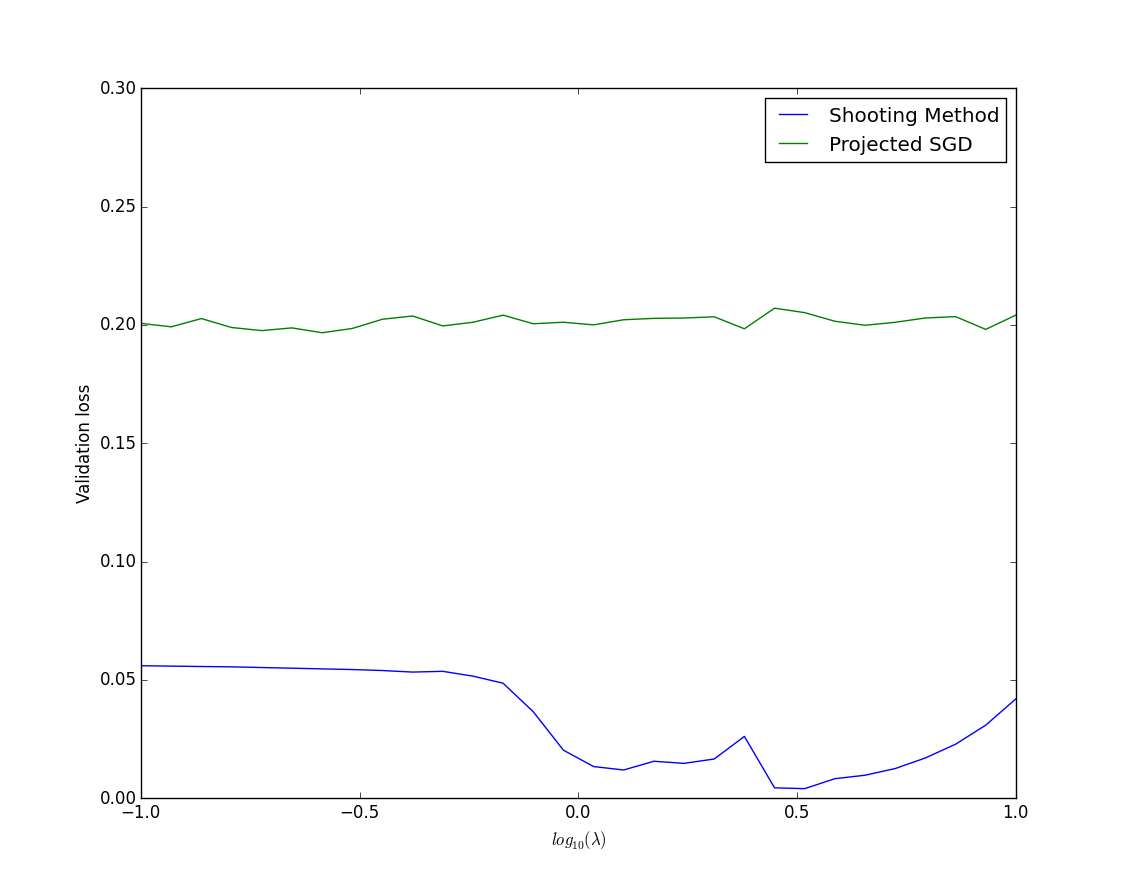
\includegraphics[width = 5in]{5_1.png}
\end{center}

From the plot we can see that, the Shooting Method have less validation loss for all different regularization parameters.  \\

\begin{problem}{5.2}
\end{problem}

According to the result, the best $\lambda$ that performed best is 0.2592. And the solution is not sparse at all. There are none zero solutions in the $\hat{w}$

\pagebreak
\begin{center}
\section{Appendix}
\end{center}
\begin{minted}{python}

def Ridge_lambda_search(X_train , y_train ,X_test, y_test, lambda_): 
	"""
	checking the convergency for different regulization lambda
	returns the last element of loss_hist returned by regularized_grad_descent
	"""

	res_training =  np.zeros(len(lambda_))
	res_testing = np.zeros(len(lambda_))
	
	for i in list(xrange(len(lambda_))):
		temp = regularized_grad_descent(X_train,y_train,lambda_reg=lambda_[i])
		theta = temp[0][-1,:]
		res_testing[i] = compute_square_loss(X_test,y_test,theta)
		res_training[i] = compute_square_loss(X_train,y_train,theta)

	return (res_testing,res_training)

def regularized_grad_descent(X, y, alpha=0.1, lambda_reg=1, num_iter=1000):

	(num_instances, num_features) = X.shape
	theta = np.ones(num_features) #Initialize theta
	theta_hist = np.zeros((num_iter+1, num_features))  #Initialize theta_hist
	loss_hist = np.zeros(num_iter+1) #Initialize loss_hist
	
	theta_hist[0,:] = theta
	loss_hist[0] = compute_square_loss(X,y,theta) + lambda_reg*np.linalg.norm(theta)**2
	
	for i in list(xrange(1,num_iter+1)):
		theta = theta - compute_regularized_square_loss_gradient(X,y,
					theta,lambda_reg)*alpha
		theta_hist[i,:] = theta 
		loss_hist[i] = compute_square_loss(X,y,theta) + 
					lambda_reg*np.linalg.norm(theta)**2

	return (theta_hist,loss_hist)  

def compute_regularized_square_loss_gradient(X, y, theta, lambda_reg):

	return compute_square_loss_gradient(X,y,theta) + 2*lambda_reg*theta 



\end{minted}




\end{document}



